\documentclass[11pt,landscape, a4paper]{extarticle}
\usepackage{multicol}
\usepackage{calc}
\usepackage{xspace}
\usepackage{xparse}
\usepackage[usenames,dvipsnames]{xcolor} 
\usepackage{ifthen}
\usepackage[landscape]{geometry}
\usepackage{hyperref}
\usepackage{tikz}
\usepackage{polynom}
\usepackage{pifont}
\usepackage{amssymb}
\usepackage{setspace}
\usepackage{dsfont}
\usepackage[italic]{derivative}
% my packages:
\usepackage{amsmath,amsfonts,amsthm,amssymb,mathrsfs,bbm,mathtools,nicefrac}\usepackage{tcolorbox}
\usepackage[utf8]{inputenc}
\usepackage{enumitem}
\usepackage{wrapfig}
%framed boxes
\usepackage{mdframed}
\usepackage{array}
\usepackage{tcolorbox}
\usepackage{accents}
\usepackage{titlesec}
\usepackage{etoolbox}
\usepackage[extreme]{savetrees}
\usepackage{wrapfig}
%for images
\usepackage{graphicx}
\geometry{a4paper, layouthoffset=0mm, margin=0mm, layoutsize={297mm, 210mm}}

\newcommand{\blankpage}{\newpage\hbox{}\thispagestyle{empty}\newpage}
\newcommand{\emptyparagraph}{\paragraph{}\noindent}

% Comments
\newcommand{\ak}[1]{{\bf[AK: #1]}}

%--------Basic Math--------
\NewDocumentCommand{\floor}{m}{\left\lfloor #1 \right\rfloor}
\NewDocumentCommand{\ceil}{m}{\left\lceil #1 \right\rceil}
\NewDocumentCommand{\ip}{m}{\left\langle #1 \right\rangle}

\newcommand*{\abs}[1]{\left| #1 \right|}
\newcommand*{\card}[1]{\left| #1 \right|}
\NewDocumentCommand{\norm}{sm}{\IfBooleanTF{#1}{\|#2\|}{\left\| #2 \right\|}}

\newcommand*{\const}{\mathrm{const}}

\newcommand*{\defeq}{\overset{.}{=}}
\newcommand*{\eqdef}{\overset{.}{=}}

\DeclareMathOperator*{\argmax}{arg\,max}
\DeclareMathOperator*{\argmin}{arg\,min}
\DeclareMathOperator*{\iid}{\smash{\overset{\mathrm{iid}}{\sim}}}

\DeclareMathOperator*{\almostsurely}{\smash{\overset{a.s.}{\rightarrow}}}
\DeclareMathOperator*{\eqalmostsurely}{\smash{\overset{a.s.}{=}}}
\DeclareMathOperator*{\convp}{\smash{\overset{\fnPr}{\rightarrow}}}
\DeclareMathOperator*{\convd}{\smash{\overset{\mathcal{D}}{\rightarrow}}}
\DeclareMathOperator*{\convms}{\smash{\overset{\ell_2}{\rightarrow}}}

\DeclarePairedDelimiter\parentheses{(}{)}
\DeclarePairedDelimiter\brackets{[}{]}
\DeclarePairedDelimiter\braces{\{}{\}}


%--------Sets--------
\newcommand{\R}{\mathbb{R}}
\newcommand{\Rzero}{\mathbb{R}_{\geq 0}}
\newcommand{\Nat}{\mathbb{N}}
\newcommand{\NatZ}{\mathbb{N}_0}


%--------Names--------
\newcommand{\MSE}{\mathrm{mse}}
\newcommand{\MLE}{\mathrm{MLE}}
\newcommand{\MAP}{\mathrm{MAP}}
\newcommand{\ls}{\mathrm{ls}}
\newcommand{\ridge}{\mathrm{ridge}}
\newcommand{\lasso}{\mathrm{lasso}}
\newcommand{\train}{\mathrm{train}}
\newcommand{\val}{\mathrm{val}}
\newcommand{\id}{\mathrm{id}}
\newcommand{\init}{\mathrm{init}}


%--------Symbols--------
\renewcommand{\vec}[1]{\mathbf{#1}}
\newcommand{\mat}[1]{\mathbf{#1}}
\newcommand{\rvec}[1]{\mathbf{#1}}
\newcommand{\set}[1]{#1}
\newcommand{\spa}[1]{\mathcal{#1}}

\newcommand{\mean}[1]{\overline{#1}}
\newcommand{\compl}[1]{\overline{#1}}
\newcommand{\old}[1]{#1^{\mathrm{old}}}
\newcommand{\opt}[1]{#1^\star}

\newcommand{\altpi}{\Pi} % \vec{\uppi}


%--------Operators--------
\NewDocumentCommand{\Ind}{m}{\mathbb{1}\{{#1}\}}
\NewDocumentCommand{\fnPr}{}{\mathbb{P}}
\RenewDocumentCommand{\Pr}{om}{\fnPr\IfValueT{#1}{_{#1}}\parentheses*{#2}}
\RenewDocumentCommand{\H}{mo}{\mathrm{H}\IfValueTF{#2}{\!\left[#1\ \middle|\ #2\right]}{\brackets*{#1}}}
\NewDocumentCommand{\Hsm}{mo}{\mathrm{H}\IfValueTF{#2}{[#1 \mid #2]}{\brackets{#1}}}
\NewDocumentCommand{\I}{mmo}{\mathrm{I}\IfValueTF{#3}{\!\left(#1;#2\ \middle|\ #3\right)}{\parentheses*{#1; #2}}}
\NewDocumentCommand{\Ism}{mmo}{\mathrm{I}\IfValueTF{#3}{(#1;#2 \mid #3)}{\parentheses{#1; #2}}}
\NewDocumentCommand{\fnS}{}{\mathrm{S}}
\RenewDocumentCommand{\S}{m}{\fnS\brackets*{#1}}
\NewDocumentCommand{\E}{somo}{\ensuremath{\mathbb{E}\IfValueT{#2}{_{#2}}{} \IfBooleanTF{#1}{#3}{\IfValueTF{#4}{\!\left[#3\ \middle|\ #4\right]}{\brackets*{#3}}}}}
\NewDocumentCommand{\Var}{somo}{\mathrm{Var}\IfValueT{#2}{_{#2}}{} \IfBooleanTF{#1}{#3}{\IfValueTF{#4}{\!\left[#3\ \middle|\ #4\right]}{\brackets*{#3}}}}
\NewDocumentCommand{\Cov}{som}{\mathrm{Cov}\IfValueT{#2}{_{#2}}{} \IfBooleanTF{#1}{#3}{\brackets*{#3}}}
\NewDocumentCommand{\Cor}{som}{\mathrm{Cor}\IfValueT{#2}{_{#2}}{} \IfBooleanTF{#1}{#3}{\brackets*{#3}}}
\NewDocumentCommand{\SD}{m}{\sigma\brackets*{#1}}
\NewDocumentCommand{\KL}{mm}{\mathrm{KL}\parentheses*{#1 \| #2}}
\NewDocumentCommand{\KLsm}{mm}{\mathrm{KL}\parentheses{#1 \| #2}}
\NewDocumentCommand{\Fisher}{mm}{\mathrm{J}\parentheses*{#1 \| #2}}
\NewDocumentCommand{\crH}{mm}{\mathrm{H}\brackets*{#1 \| #2}}
\NewDocumentCommand{\crHsm}{mm}{\mathrm{H}\brackets{#1 \| #2}}

\NewDocumentCommand{\fnv}{oo}{v\IfValueT{#2}{_{#2}}\IfValueT{#1}{^{#1}}}
\RenewDocumentCommand{\v}{somo}{\IfBooleanTF{#1}{\fnv[\star][#4]\parentheses{#3}}{\fnv[#2][#4]\parentheses{#3}}}
\NewDocumentCommand{\fnq}{oo}{q\IfValueT{#2}{_{#2}}\IfValueT{#1}{^{#1}}}
\NewDocumentCommand{\q}{sommo}{\IfBooleanTF{#1}{\fnq[\star][#5]\parentheses{#3,#4}}{\fnq[#2][#5]\parentheses{#3,#4}}}
\NewDocumentCommand{\fnV}{oo}{V\IfValueT{#2}{_{#2}}\IfValueT{#1}{^{#1}}}
\NewDocumentCommand{\V}{somo}{\IfBooleanTF{#1}{\fnV[\star][#4]\parentheses{#3}}{\fnV[#2][#4]\parentheses{#3}}}
\NewDocumentCommand{\fnQ}{oo}{Q\IfValueT{#2}{_{#2}}\IfValueT{#1}{^{#1}}}
\NewDocumentCommand{\Q}{sommo}{\IfBooleanTF{#1}{\fnQ[\star][#5]\parentheses{#3,#4}}{\fnQ[#2][#5]\parentheses{#3,#4}}}
\NewDocumentCommand{\fna}{oo}{a\IfValueT{#2}{_{#2}}\IfValueT{#1}{^{#1}}}
\RenewDocumentCommand{\a}{sommo}{\IfBooleanTF{#1}{\fna[\star][#5]\parentheses{#3,#4}}{\fna[#2][#5]\parentheses{#3,#4}}}
\NewDocumentCommand{\fnA}{oo}{A\IfValueT{#2}{_{#2}}\IfValueT{#1}{^{#1}}}
\NewDocumentCommand{\A}{sommo}{\IfBooleanTF{#1}{\fnA[\star][#5]\parentheses{#3,#4}}{\fnA[#2][#5]\parentheses{#3,#4}}}
\RenewDocumentCommand{\j}{mo}{j\IfValueT{#2}{_{#2}}\parentheses{#1}}
\NewDocumentCommand{\fnJ}{o}{J\IfValueT{#1}{_{#1}}}
\NewDocumentCommand{\J}{mo}{\fnJ[#2]\parentheses{#1}}

\NewDocumentCommand{\pset}{m}{\mathcal{P}\parentheses*{#1}}

\NewDocumentCommand{\pf}{mm}{{#1}_\sharp #2}

\NewDocumentCommand{\grad}{e_}{\boldsymbol{\nabla}\IfValueT{#1}{_{\!\!#1}\,}}
\NewDocumentCommand{\jac}{}{\mD}
\NewDocumentCommand{\hes}{}{\mH}
\NewDocumentCommand{\dive}{}{\grad\cdot}
\NewDocumentCommand{\lapl}{}{\Delta}

\NewDocumentCommand{\BigO}{m}{\mathcal{O}\parentheses*{#1}}
\NewDocumentCommand{\BigOTil}{m}{\Tilde{\mathcal{O}}\parentheses*{#1}}

\NewDocumentCommand{\transpose}{m}{#1^\top}
\NewDocumentCommand{\inv}{m}{#1^{-1}}
\RenewDocumentCommand{\det}{m}{\mathrm{det}\parentheses*{#1}}
\NewDocumentCommand{\tr}{m}{\mathrm{tr}\parentheses*{#1}}
\NewDocumentCommand{\diag}{om}{\mathrm{diag}\IfValueT{#1}{_{#1}}{}\braces{#2}}
\NewDocumentCommand{\msqrt}{m}{#1^{\nicefrac{1}{2}}}
\NewDocumentCommand{\vecop}{m}{\mathrm{vec}\brackets{#1}}

\NewDocumentCommand{\N}{somm}{\mathcal{N}\IfBooleanTF{#1}{\left(}{(}\IfValueT{#2}{#2;}{} #3, #4\IfBooleanTF{#1}{\right)}{)}}
\NewDocumentCommand{\SN}{o}{\mathcal{N}(\IfValueT{#1}{#1;}{} \vzero, \mI)}
\NewDocumentCommand{\uSN}{o}{\mathcal{N}(\IfValueT{#1}{#1;}{} 0, 1)}
\NewDocumentCommand{\KF}{ommmmm}{\mathcal{KF}(\IfValueT{#1}{#1;}{} #2, #3, #4, #5, #6)}
\NewDocumentCommand{\GP}{omm}{\mathcal{GP}(\IfValueT{#1}{#1;}{} #2, #3)}
\NewDocumentCommand{\Unif}{om}{\mathrm{Unif}(\IfValueT{#1}{#1;}{} #2)}
\NewDocumentCommand{\Bern}{om}{\mathrm{Bern}(\IfValueT{#1}{#1;}{} #2)}
\NewDocumentCommand{\Bin}{omm}{\mathrm{Bin}(\IfValueT{#1}{#1;}{} #2, #3)}
\NewDocumentCommand{\Beta}{omm}{\mathrm{Beta}(\IfValueT{#1}{#1;}{} #2, #3)}
\NewDocumentCommand{\Laplace}{omm}{\mathrm{Laplace}(\IfValueT{#1}{#1;}{} #2, #3)}
\NewDocumentCommand{\Cauchy}{omm}{\mathrm{Cauchy}(\IfValueT{#1}{#1;}{} #2, #3)}
\NewDocumentCommand{\GammaDistr}{omm}{\mathrm{Gamma}(\IfValueT{#1}{#1;}{} #2, #3)}
\NewDocumentCommand{\Pareto}{omm}{\mathrm{Pareto}(\IfValueT{#1}{#1;}{} #2, #3)}

\newcommand{\sigman}{\sigma_{\mathrm{n}}}
\newcommand{\sigmap}{\sigma_{\mathrm{p}}}


%--------Common vectors/matrices/sets--------
\newcommand{\vzero}{\vec{0}}
\newcommand{\vone}{\vec{1}}
\newcommand{\va}{\vec{a}}
\newcommand{\vap}{\vec{a'}}
\newcommand{\vas}{\vec{\opt{a}}}
\newcommand{\vb}{\vec{b}}
\newcommand{\vc}{\vec{c}}
\newcommand{\vd}{\vec{d}}
\newcommand{\ve}{\vec{e}}
\newcommand{\vf}{\vec{f}}
\newcommand{\vfhat}{\vec{\hat{f}}}
\newcommand{\vg}{\vec{g}}
\newcommand{\vk}{\vec{k}}
\newcommand{\vm}{\vec{m}}
\newcommand{\vp}{\vec{p}}
\newcommand{\vq}{\vec{q}}
\newcommand{\vr}{\vec{r}}
\newcommand{\vs}{\vec{s}}
\newcommand{\vt}{\vec{t}}
\newcommand{\vu}{\vec{u}}
\newcommand{\vv}{\vec{v}}
\newcommand{\vvp}{\vec{v'}}
\newcommand{\vvs}{\vec{\opt{v}}}
\newcommand{\vw}{\vec{w}}
\newcommand{\vwhat}{\vec{\hat{w}}}
\newcommand{\vx}{\vec{x}}
\newcommand{\vxp}{\vec{x'}}
\newcommand{\vxs}{\vec{\opt{x}}}
\newcommand{\vy}{\vec{y}}
\newcommand{\vyp}{\vec{y'}}
\newcommand{\vz}{\vec{z}}
\newcommand{\valpha}{\vec{\alpha}}
\newcommand{\valphahat}{\vec{\hat{\alpha}}}
\newcommand{\vdelta}{\vec{\delta}}
\newcommand{\vDelta}{\vec{\Delta}}
\newcommand{\vepsilon}{\vec{\epsilon}}
\newcommand{\veta}{\vec{\eta}}
\newcommand{\vlambda}{\vec{\lambda}}
\newcommand{\vmu}{\vec{\mu}}
\newcommand{\vmuhat}{\vec{\hat{\mu}}}
\newcommand{\vmup}{\vec{\mu'}}
\newcommand{\vnu}{\vec{\nu}}
\newcommand{\vomega}{\vec{\omega}}
\newcommand{\vphi}{\vec{\phi}}
\newcommand{\vpi}{\vec{\pi}}
\newcommand{\vpsi}{\vec{\psi}}
\newcommand{\vvarphi}{\vec{\varphi}}
\newcommand{\vvarphihat}{\vec{\hat{\varphi}}}
\newcommand{\vtheta}{\vec{\theta}}
\newcommand{\vthetahat}{\vec{\hat{\theta}}}
\newcommand{\vxi}{\vec{\xi}}
\newcommand{\mzero}{\mat{0}}
\newcommand{\mA}{\mat{A}}
\newcommand{\mB}{\mat{B}}
\newcommand{\mBs}{\mat{\opt{B}}}
\newcommand{\mC}{\mat{C}}
\newcommand{\mD}{\mat{D}}
\newcommand{\mF}{\mat{F}}
\newcommand{\mH}{\mat{H}}
\newcommand{\mI}{\mat{I}}
\newcommand{\mK}{\mat{K}}
\newcommand{\mL}{\mat{L}}
\newcommand{\mCalL}{\mat{\mathcal{L}}}
\newcommand{\mM}{\mat{M}}
\newcommand{\mP}{\mat{P}}
\newcommand{\mQ}{\mat{Q}}
\newcommand{\mS}{\mat{S}}
\newcommand{\mT}{\mat{T}}
\newcommand{\mU}{\mat{U}}
\newcommand{\mV}{\mat{V}}
\newcommand{\mW}{\mat{W}}
\newcommand{\mX}{\mat{X}}
\newcommand{\mLambda}{\mat{\Lambda}}
\newcommand{\mPhi}{\mat{\Phi}}
\newcommand{\mPi}{\mat{\Pi}}
\newcommand{\mSigma}{\mat{\Sigma}}
\newcommand{\mSigmap}{\mat{\Sigma'}}
\newcommand{\rG}{\rvec{G}}
\newcommand{\rQ}{\rvec{Q}}
\newcommand{\rU}{\rvec{U}}
\newcommand{\rV}{\rvec{V}}
\newcommand{\rW}{\rvec{W}}
\newcommand{\rX}{\rvec{X}}
\newcommand{\rXp}{\rvec{X'}}
\newcommand{\rY}{\rvec{Y}}
\newcommand{\rZ}{\rvec{Z}}
\newcommand{\sA}{\set{A}}
\newcommand{\sB}{\set{B}}
\newcommand{\sC}{\set{C}}
\newcommand{\sD}{\set{D}}
\newcommand{\sI}{\set{I}}
\newcommand{\sM}{\set{M}}
\newcommand{\sS}{\set{S}}
\newcommand{\sU}{\set{U}}
\newcommand{\sX}{\set{X}}
\newcommand{\sY}{\set{Y}}
\newcommand{\sZ}{\set{Z}}
\newcommand{\spA}{\spa{A}}
\newcommand{\spB}{\spa{B}}
\newcommand{\spC}{\spa{C}}
\newcommand{\spD}{\spa{D}}
\newcommand{\spF}{\spa{F}}
\newcommand{\spH}{\spa{H}}
\newcommand{\spM}{\spa{M}}
\newcommand{\spO}{\spa{O}}
\newcommand{\spP}{\spa{P}}
\newcommand{\spQ}{\spa{Q}}
\newcommand{\spT}{\spa{T}}
\newcommand{\spX}{\spa{X}}
\newcommand{\spY}{\spa{Y}}
\newcommand{\spZ}{\spa{Z}}
\newcommand{\fs}{\opt{f}}
\newcommand{\ps}{\opt{p}}
\newcommand{\qs}{\opt{q}}
\newcommand{\xs}{\opt{x}}
\newcommand{\ys}{\opt{y}}
\newcommand{\Bs}{\opt{B}}
\newcommand{\Qs}{\opt{Q}}
\newcommand{\sSs}{\opt{\sS}}
\newcommand{\hQs}{\opt{\hat{Q}}}
\newcommand{\Vs}{\opt{V}}
\newcommand{\pis}{\opt{\pi}}

\newcommand{\vF}{\rvec{F}}
\newcommand{\vS}{\rvec{S}}
\newcommand{\vT}{\rvec{T}}



% Turn off header and footer
\pagestyle{plain}
% Turn off page numbering
\pagenumbering{gobble}

% Redefine section commands to use less space
\titleformat{name=\section}[block]
  {\sffamily\scriptsize}
  {}
  {0pt}
  {\colorsection}
\titlespacing*{\section}{0mm}{-1mm}{-1mm}
%\makeatletter

\newcommand{\colorsection}[1]{%
  \colorbox{blue!20}{{\thesection\ #1}}}

%\renewcommand{\section}{\@startsection{section}{1}{0mm}%
                                %{-1ex plus -.5ex minus -.2ex}%
                                %{0.5ex plus .2ex}%x
                                %{\normalfont\small\bfseries}}
%\makeatother

% Don't print section numbers
\setcounter{secnumdepth}{1}

\setlength{\parindent}{0pt}
\setlength{\parskip}{0pt}
% define box
\tikzstyle{fancytitle} =[fill=black, text=white, font=\footnotesize\bfseries]

\definecolor{light}{rgb}{0.5, 0.5, 0.5}
\definecolor{background_color}{HTML}{7D98A1}
\def\light#1{{\color{light}#1}}

% -----------------------------------------------------------------------
\setstretch{-0.6} %Line spacing
\makeatletter
\patchcmd\set@fontsize{#3}{#2}{}{}
\makeatother
\begin{document}
\raggedright
\footnotesize
\setlength{\columnseprule}{0.25pt}
\setlength{\premulticols}{1pt}
\setlength{\postmulticols}{1pt}
\setlength{\multicolsep}{-1cm}
\setlength{\columnsep}{1mm}
\begin{multicols*}{5}

% multicol parameters
% These lengths are set only within the two main columns



% main heading
\begin{center}
	\Large{\textbf{Probablistic AI}} \\
\end{center}
\vspace{-4mm}
\newcommand\Reihe{\sum_{k = 1}^{\infty}}

\newcommand\Ib{\overline{I}}

\newcommand*\diff{\mathop{}\!\mathrm{d}}

\newcommand\Title[1]{\vspace{.1mm}\begin{tikzpicture} \node[fancytitle, right=10pt, fill=gray] {#1}; \end{tikzpicture}}

%\everymath{\color{PineGreen}}
\definecolor{math}{HTML}{0047AB}
\everymath{\color{math}}
\newcommand{\ubar}[1]{\underaccent{\bar}{#1}}

%\renewcommand{\(}{\relax\ifmmode\@badmath\else\color{blue}$\fi}
%\renewcommand{\)}{\relax\ifmmode\ifinner$\color{black}\else\@badmath\fi\else \@badmath\fi }
%\catcode`\$=13
%\def${\ifmmode)\xspace\else(\fi} 
%\makeatother

\scriptsize

\newenvironment{framed}
{\vspace{0.5mm}\begin{tcolorbox}[colback=background_color!15!white,
                   colframe=black, 
                   boxrule=0.3pt,
                   enlarge top by=0cm, 
                   enlarge bottom by=0cm, 
                   enlarge left by=0cm,
                   left=6pt,
                   right=6pt,
                   boxsep=-2mm]}
		{\end{tcolorbox}\vspace{0.5mm}}

% _____ BEGINNING OF DOCUMENT __________________________________________________

\section{Fundamentals}
\begin{framed}
    \textbf{Useful PDFs:} \\
    \textbf{Normal}:$\frac{\exp \left(-\frac{1}{2}(\vx - \vmu)^T \Sigma^{-1} (\vx - \vmu) \right)}{\sqrt{(2\pi)^k \det{\Sigma}}}$ \\
    \textbf{Beta}: $\Beta[\theta]{\alpha}{\beta} \propto \theta^{\alpha-1} (1-\theta)^{\beta-1}$ \\
    \textbf{Laplace}: $\frac{1}{2l}\exp\left(-\frac{\abs{x - \mu}}{l}\right)$
\end{framed}
\begin{framed}
    \textbf{Properties of Expectation:}\\
    $\E{\mA \rX + \vb} = \mA \E{\rX} + \vb $\\ 
    $ \E{\rX + \rY} = \E{\rX} + \E{\rY}$ \\
    $\E{\rX\transpose{\rY}} = \E{\rX} \cdot \transpose{\E{\rY}}$ (if independent)\\
    $\E[\rY]{\E[\rX]{\rX \mid \rY}} = \E{\rX}$ (\textbf{Tower rule})
\end{framed} 
\begin{framed}
    \textbf{Variance and Covariance}\\
    $\rX \in \R^n$, $\rY \in \R^m$ random vectors.\\
    $\Cov{\rX, \rY} \defeq \E{(\rX - \E{\rX})\transpose{(\rY - \E{\rY})}}$\\
    $\Cov{\mA \rX + \vc, \mB \rY + \vd} = \mA \Cov{\rX, \rY} \transpose{\mB}$\\
    \emph{Uncorrelated} if and only if $\Cov{\rX, \rY} = \mzero$.\\
    The \emph{correlation} of the random vectors $\rX$ and $\rY$ is a normalized covariance: 
    $\Cor{\rX, \rY}(i,j) \defeq \frac{\Cov{X_i, Y_j}}{\sqrt{\Var{X_i} \Var{Y_j}}} \in [-1, 1]$\\
    $\Var{\rX} \defeq \Cov{\rX, \rX}$\\
    $\text{Var}(X+Y) = \text{Var}(X) + \text{Var}(Y) + 2\text{Cov}(X, Y)$\\
    $\text{Var}(X-Y) = \text{Var}(X) + \text{Var}(Y) - 2\text{Cov}(X, Y)$\\
\end{framed}

\begin{framed}
    \textbf{Inverse of a 2x2 matrix}\\
    $\mA=\begin{pmatrix}a&b\\c&d\end{pmatrix}, \mA^{-1}=\frac{1}{ad-bc}\begin{pmatrix}d&-b\\-c&a\end{pmatrix}$
\end{framed}
\begin{framed}
    \textbf{Frobenius Norm}\\
    \(\norm{\mA}_F=\sqrt{\sum_{i=1}^{m}{\sum_{j=1}^{n}{a_{ij}^2}}}\)
\end{framed}
\begin{framed}
\textbf{Properties of variance}:\\
$\Var{\mA\rX + \vb} = \mA\Var{\rX}\transpose{\mA}$\\
$\Var{\rX + \rY} = \Var{\rX} + \Var{\rY} + 2 \Cov{\rX, \rY}$\\
$\Var{\rX + \rY} = \Var{\rX} + \Var{\rY}$ (if $\rX$, $\rY$ independant)
$\Var{\rX} = \E[\rY]{\Var[\rX]{\rX \mid \rY}} + \Var[\rY]{\E[\rX]{\rX \mid \rY}}$ (\textbf{Law of total variance})
\end{framed}
\textbf{Change of variables formula}
Let $\vg$ be differentiable and invertible. Then for $\rY = \vg(\rX)$ we have $p_\rY(\vy) = p_\rX(\inv{\vg}(\vy)) \cdot \abs{\det{\jac \inv{\vg}(\vy)}}$ where $\jac \inv{\vg}(\vy)$ is the Jacobian of $\inv{\vg}$ evaluated at $\vy$.
\begin{framed}
\textbf{Bayes' rule}: 
$p(\vx \mid \vy) = \frac{p(\vy \mid \vx) \cdot p(\vx)}{p(\vy)}$ \\
$P(A \mid B, C) = \frac{P(B \mid A, C) P(A \mid C)}{P(B \mid C)}$


\end{framed}
\begin{framed}
    \textbf{Posterior} $p(\vx \mid \vy)$: updated belief about $\vx$ after observing $\vy$. \\
    \textbf{Prior} $p(\vx)$: initial belief about $\vx$. \\
    \textbf{Conditional likelihood} $p(\vy \mid \vx)$: how likely the observations $\vy$ are under a given value $\vx$. \\
    \textbf{Joint likelihood} $p(\vx, \vy) = p(\vy \mid \vx) p(\vx)$ \\
    \textbf{Marginal likelihood} $p(\vy)$: how likely the observations $\vy$ are across all values of $\vx$. \\
    \textbf{Marginal likelihood} $p(\vy) = \int_{\rX(\Omega)} p(\vy \mid \vx) \cdot p(\vx) \,d\vx$. 
\end{framed}
If prior $p(\vx)$ and posterior $p(\vx \mid \vy)$ from same family of distributions, the prior is a \textbf{conjugate prior} to the likelihood $p(\vy \mid \vx)$. The beta distribution is a conjugate prior to a binomial likelihood. \\
\begin{framed}
    \textbf{Normal Distribution} \\
    $\rX\sim\N{\vmu}{\mSigma}$. $\mA\rX+\vb\sim\N{\mA\mu+\vb,\mA\mSigma \mA^T}$.\\
    Let $\rX$ be Gaussian and index sets $\sA, \sB \subseteq [n]$.
    For any such \textbf{marginal distribution} $\rX_A \sim \N{\vmu_\sA}{\mSigma_{\sA\sA}}$ and that for any such \textbf{conditional distribution}: \\
    $ \rX_\sA \mid \rX_\sB = \vx_\sB \sim \N{\vmu_{\sA \mid \sB}}{\mSigma_{\sA \mid \sB}}$ where: \\
        $\vmu_{\sA \mid \sB} \defeq \vmu_\sA + \mSigma_{\sA\sB}\inv{\mSigma_{\sB\sB}}(\vx_\sB - \vmu_\sB)$ and \\
        $\mSigma_{\sA \mid \sB} \defeq \mSigma_{\sA\sA} - \mSigma_{\sA\sB}\inv{\mSigma_{\sB\sB}}\mSigma_{\sB\sA}$.
\end{framed}
\textbf{Maximum likelihood estimate (MLE)}: $\vthetahat_\MLE \defeq$
 $\underset{\vtheta \in \Theta}{\argmax}\ p(y_{1:n} \mid \vx_{1:n}, \vtheta) 
  = \underset{\vtheta \in \Theta}{\argmax}\ \underbrace{\sum_{i=1}^n \log p(y_i \mid \vx_i, \vtheta)}_{\text{{log-likelihood}}}$ \\
$\ell_\mathrm{nll}(\vtheta; \spD_n)$: negative log-likelihood
The MLE is \textbf{consistent} and \textbf{asymptotically normal} if: $\vthetahat_\MLE \convp \opt{\vtheta}$ $\vthetahat_\MLE \convd \N{\opt{\vtheta}}{\mS_n}$ as $n \to \infty$. \\
\textbf{{Maximum A Posteriori (MAP) estimate}}:   $\vthetahat_\MAP \defeq \argmax_{\vtheta \in \Theta} p(\vtheta \mid \vx_{1:n}, y_{1:n}) 
  = \argmin_{\vtheta \in \Theta} \underbrace{- \log p(\vtheta)}_{\text{regularization}} + \underbrace{\ell_\mathrm{nll}(\vtheta; \spD_n)}_{\text{quality of fit}}$
\begin{framed}
\textbf{Common regularizers}: \\
 $p(\vtheta) = \N[\vtheta]{\vzero}{\lambda \mI}$ $\rightarrow$ $-\log p(\vtheta) = \frac{\lambda}{2} \norm{\vtheta}_2^2 + \const$ \\
 $p(\vtheta) = \Laplace[\vtheta]{\vzero}{\lambda}$ $\rightarrow$ $-\log p(\vtheta) = \lambda \norm{\vtheta}_1 + \const$,
 uniform prior $\rightarrow$ $\const$
 \end{framed}
\begin{framed}
     \textbf{Expected calibration error}: For $m$ bins: $\ell_{\mathrm{ECE}} \defeq \sum_{m=1}^M \frac{\card{\sB_m}}{n} \abs{\mathrm{freq}(\sB_m) - \mathrm{conf}(\sB_m)}$
 \end{framed}


\section{Bayesian Linear Regression}
\begin{framed}
    \textbf{Closed form solutions}:
    $\vwhat_{\ls} = \inv{(\transpose{\mX} \mX)} \transpose{\mX} \vy$  \\
    $\vwhat_{\ridge} = \inv{(\transpose{\mX} \mX + \lambda \mI)} \transpose{\mX} \vy$
\end{framed}
\textbf{Notable Results}: $\Var{\vwhat_{\ls} \mid \rX} = \sigman^2(\transpose{\rX}\rX)^{-1}$ \\
A \textbf{Gaussian prior on the weights} $\vw \sim \N{\vzero}{\sigmap^2 \mI}$, yields the posterior distribution: $\log p(\vw \mid \vx_{1:n}, y_{1:n}) = -\frac{1}{2} \brackets*{\transpose{\vw}\mSigma^{-1}\vw - 2\vmu} + \const$, with $\mSigma \defeq \inv{\parentheses*{\sigman^{-2} \transpose{\mX} \mX + \sigmap^{-2} \mI}}$ and $\vmu \defeq \sigman^{-2} \mSigma \transpose{\mX} \vy$. We have $\vw \mid \vx_{1:n}, y_{1:n} \sim \N{\vmu}{\mSigma}$: \textit{Gaussian's with known variance and linear likelihood} are self-conjugate. \\
MAP: $\vwhat_\MAP = \argmin_\vw \norm{\vy - \mX \vw}_2^2 + \frac{\sigman^2}{\sigmap^2} \norm{\vw}_2^2$, \textit{identical to ridge regression} with $\lambda \defeq \sigman^2 / \sigmap^2$. \\
A \textbf{Laplace prior} on the weights is equivalent to \textbf{lasso regression} with decay ${\lambda \defeq \sigman^2 / \ell}$. \\
\textbf{Bayesian inference}: Distribution for a test point $\vxs$ is: $\ys \mid \vxs, \vx_{1:n}, y_{1:n} \sim \N{\transpose{\vmu} \vxs}{\transpose{\vxs} \mSigma \vxs + \sigman^2}$. \\
$\Var{\ys \mid \vxs} = \underbrace{\E[\vtheta]{\Var[\ys]{\ys \mid \vxs, \vtheta}}}_{\text{aleatoric uncertainty}} + \underbrace{\Var[\vtheta]{\E[\ys]{\ys \mid \vxs, \vtheta}}}_{\text{epistemic uncertainty}}$.\\
Aleatoric $\rightarrow$ noise in data; Epistemic $\rightarrow$ noise in model.
Applying linear regression to non linear functions: apply a non linear transformation $\vphi$ to $\rX$. Define $\mPhi = \vphi(\rX)$, so-called \textbf{Kernel}. With a gaussian prior we get: $\vf \mid \mX \sim \N{\mPhi \E{\vw}}{\mPhi \Var{\vw} \transpose{\mPhi}} = \N{\vzero}{\mK}$, with $\mK = \sigmap^2 \mPhi \transpose{\mPhi}$. We define the \textbf{Kernel-function}: $k(\vx, \vxp) \defeq \sigmap^2 \cdot \transpose{\vphi(\vx)} \vphi(\vxp) = \Cov{f(\vx), f(\vxp)}$.
\begin{framed}
    \textbf{Linear Kernel}: $k(\vx, \vxp) = l \transpose{\vx} \vxp$ \\
    \textbf{RBF/Gaussian}: $k(\vx, \vxp) = \exp{-\frac{(\vx - \vxp)^2}{2\sigma_p^2}}$ \\
    \textbf{Polynomial Kernel} $k(\vx, \vxp) = (1 + \transpose{\vx} \vxp)^d$ \\
    \textbf{Laplacian kernel}: $k(\vx, \vxp) = \exp{\left(-\alpha \norm{\vx - \vxp}\right)}$
\end{framed}
\begin{framed}
    \textbf{Properties of Kernels}:  \\
    Symmetry: $k(\vx, \vxp) = k(\vxp, \vx)$ and $\mK_{\sA\sA}$ is p.s.d. \\
    Kernels can be \textbf{composed} in the following ways to obtain a new kernel: addition, multiplication, positive scalar multiplication and composition with a funtion $f$ if $f$ is polynomial with positive coefficients or $\exp$.
\end{framed}
\textbf{Stationary} if there exists a $\tilde{k}$ s.t. $\tilde{k}(\vx - \vxp) = k(\vx, \vxp)$, and \textbf{Isotropic} if there exists a $\tilde{k}$ s.t. $\tilde{k}(\norm{\vx-\vxp}_2) = k(\vx, \vxp)$.


\section{Gaussian Processes}
\begin{framed}
    A Gaussian process is characterized by a \textbf{mean function} $\mu : \spX \to \R$ and a \textbf{covariance function} (or \textbf{kernel function}) $k : \spX \times \spX \to \R$ such that for any $\sA \defeq \{\vx_1, \dots, \vx_m\} \subseteq \spX$, we have 
  $\vf_\sA \defeq \transpose{[f_{\vx_1} \; \cdots \; f_{\vx_m}]} \sim \N{\vmu_\sA}{\mK_{\sA\sA}}$ 
We write $f \sim \GP{\mu}{k}$.
In particular,  
  $\ys \mid \vxs, \mu, k \sim \N{\mu(\vxs)}{k(\vxs, \vxs) + \sigman^2}$ (homoscedastic noise)
\end{framed}
\begin{framed}
    \textbf{Maximize Marginal Likelihood}: \\
    $ \vthetahat_\MLE \defeq \argmax_{\vtheta} p(y_{1:n} \mid \vx_{1:n}, \vtheta) \\= \argmax_{\vtheta} \int p(y_{1:n} \mid \vx_{1:n}, f, \vtheta) p(f \mid \vtheta) \,d f$.
\end{framed}
\textbf{Update:} Joint distribution of the observations $y_{1:n}$ and the noise-free prediction $\fs$ at a test point $\vxs$ as $\begin{bmatrix}
    \vy \\
    \fs \\
  \end{bmatrix} \mid \vxs, \vx_{1:n} \sim \N{\Tilde{\vmu}}{\Tilde{\mK}}$ \\
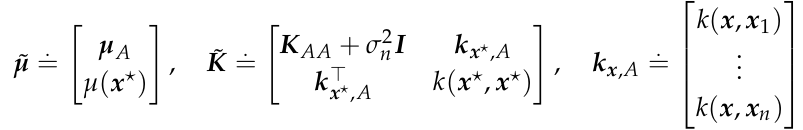
\includegraphics[width=\linewidth]{images/GP_Update}
\textbf{GP posterior}: 
$f \mid \vx_{1:n}, y_{1:n} \sim \GP{\mu'}{k'}$ where $
  \mu'(\vx) \defeq \mu(\vx) + \transpose{\vk_{\vx,\sA}} \inv{(\mK_{\sA\sA} + \sigman^2 \mI)} (\vy_\sA - \vmu_\sA)$ and $
  k'(\vx, \vxp) \defeq k(\vx, \vxp) - \transpose{\vk_{\vx,\sA}} \inv{(\mK_{\sA\sA} + \sigman^2 \mI)} \vk_{\vxp,\sA}$
For GP-Regression ($y_{1:n} \mid \vx_{1:n}, \vtheta \sim \N{\vzero}{\mK_{f,\vtheta} + \sigman^2 \mI}$), write $\mK_{\vy,\vtheta} \defeq \mK_{f,\vtheta} + \sigman^2 \mI$, and obtain: $\vthetahat_\MLE = \argmin_{\vtheta} \frac{1}{2} \transpose{\vy} \inv{\mK_{\vy,\vtheta}} \vy + \frac{1}{2} \log \det{\mK_{\vy,\vtheta}}$. Also:
$\pdv{}{\theta_j} \log p(y_{1:n} \mid \vx_{1:n}, \vtheta) = \frac{1}{2} \tr{(\valpha \transpose{\valpha} - \inv{\mK_{\vy,\vtheta}}) \pdv{\mK_{\vy,\vtheta}}{\theta_j}}$.\\
\textbf{Approximations}: Gaussian process need to invert Matrices $\rightarrow$ computational cost of $\BigO{n^3}$. \\ 
\textbf{Local method}: When sampling at $\vx$ only condition on the samples $\vxp$, that are close, i.e. where $\abs{k(\vx, \vxp)} \geq \tau$ for some $\tau > 0$, instead of all samples. \textbf{Problem:} $\tau$ has to be chosen carefully: if $\tau$ is chosen too large, samples become essentially independent. \\
\textbf{Kernel Approximation}: Construct a low dimensional feature map $\vphi : \R^d \to \R^m$ that approximates the kernel: $k(\vx, \vxp) \approx \transpose{\vphi(\vx)} \vphi(\vxp)$. Then apply Bayesian linear regression $\rightarrow$ time complexity of $\BigO{n m^2 + m^3}$. This can be done with \textbf{Random Fourier features}: a \textit{stationary} kernel $k$ can be interpreted as a function in one variable, and has an associated Fourier transform which we denote by $p(\vomega)$: $k(\vx-\vxp) = \int_{\R^d} p(\vomega) e^{i \transpose{\vomega} (\vx-\vxp)} \,d\vomega$.
\begin{framed}
    \textbf{Bochner's Theorem} A continuous Kernel on $\R^d$ is p.s.d iff its Fourier transform $p(\vomega)$ is non-negative.
\end{framed}
$\implies$ If continuous and stationary kernel is p.s.d. and scaled correctly then $p(\vomega)$ is a probability distribution named \textbf{spectral density} of $k$. The spectral density can be computed by: $p(\vomega) = \int_{\R^d} k(\vomega) e^{- i 2 \pi \transpose{\vxi} \vomega} \,d\vomega.$ \\ Now write the kernel as an expectation: $k(\vx-\vxp) = \int_{\R^d} p(\vomega) e^{i \transpose{\vomega} (\vx-\vxp)} \,d\vomega = \E[\vomega \sim p]{e^{i \transpose{\vomega}(\vx-\vxp)}}= \transpose{\vz(\vx)} \vz(\vxp)$, where $z_{\vomega,b}(\vx) \defeq \sqrt{2} \cos(\transpose{\vomega} \vx + b)$, and $\vz(\vx) \defeq \frac{1}{\sqrt{m}} \transpose{[z_{\vomega^{(1)},b^{(1)}}(\vx), \dots, z_{\vomega^{(m)},b^{(m)}}(\vx)]}$ is a randomized feature map of Fourier transforms $\vomega^{(i)} \iid p$ and $b^{(i)} \iid \Unif{\brackets{0, 2 \pi}}$. The error probability decays exponentially in $\epsilon$.
\begin{framed}
    \textbf{Inducing Points}    
    SoR/FITC: runtime \(\mathcal{O}(n^3)\) in number of inducing points, \(\mathcal{O}(n)\) in number of points. Inducing points can be seen as hyperparameters to optimize.
\end{framed}
\begin{framed}
  \textbf{Kalman Filter}\\
  $\mathbf{X}_{t+1} \perp \mathbf{X}_{1:t-1} \mid \mathbf{X}_t, \quad \mathbf{Y}_t \perp \mathbf{Y}_{1:t-1} \mid \mathbf{X}_t$\\
  $P(\mathbf{X}_1) \sim \mathcal{N}(\boldsymbol{\mu}, \boldsymbol{\Sigma})$\\
  \textbf{Motion:} $P(\mathbf{X}_{t+1} \mid \mathbf{X}_t) = \mathcal{N}(\mathbf{F} \mathbf{X}_t, \boldsymbol{\Sigma}_x)$, \quad $\mathbf{X}_{t+1} = \mathbf{F} \mathbf{X}_t + \epsilon_t$\\
  \textbf{Sensor:} $P(\mathbf{Y}_t \mid \mathbf{X}_t) = \mathcal{N}(\mathbf{H} \mathbf{X}_t, \boldsymbol{\Sigma}_y)$, \quad $\mathbf{Y}_t = \mathbf{H} \mathbf{X}_t + \eta_t$\\
  \textbf{Update:} $\boldsymbol{\mu}_{t+1} = \mathbf{F} \boldsymbol{\mu}_t + \mathbf{K}_{t+1}(\mathbf{y}_{t+1} - \mathbf{H} \mathbf{F} \boldsymbol{\mu}_t)$, \\
  $\boldsymbol{\Sigma}_{t+1} = (\mathbf{I} - \mathbf{K}_{t+1} \mathbf{H})(\mathbf{F} \boldsymbol{\Sigma}_t \mathbf{F}^\top + \boldsymbol{\Sigma}_x)$\\
  \textbf{Gain:} $\mathbf{K}_{t+1} = (\mathbf{F} \boldsymbol{\Sigma}_t \mathbf{F}^\top + \boldsymbol{\Sigma}_x) \mathbf{H}^\top [\mathbf{H}(\mathbf{F} \boldsymbol{\Sigma}_t \mathbf{F}^\top + \boldsymbol{\Sigma}_x)\mathbf{H}^\top + \boldsymbol{\Sigma}_y]^{-1}$\\
  \textbf{Filtering:}\\
  $P(\mathbf{X}_t \mid \mathbf{y}_{1:t}) = \frac{1}{Z} P(\mathbf{y}_t \mid \mathbf{X}_t) P(\mathbf{X}_t \mid \mathbf{y}_{1:t-1})$, \\
  $P(\mathbf{X}_{t+1} \mid \mathbf{y}_{1:t}) = \int P(\mathbf{X}_{t+1} \mid \mathbf{X}_t) P(\mathbf{X}_t \mid \mathbf{y}_{1:t}) d\mathbf{X}_t$
\end{framed}

\section{Variational Inference}
Approximate the true posterior distribution with a simpler posterior that is easy to sample: \\$p(\vtheta \mid \vx_{1:n}, y_{1:n}) = \frac{1}{Z} p(\vtheta, y_{1:n} \mid \vx_{1:n}) \approx q(\vtheta \mid \vlambda) \eqdef q_\vlambda(\vtheta)$, where $\vlambda$ represents the parameters of the \textbf{variational posterior} $q_\vlambda$.\\
\textbf{Laplace Approximation}: Idea: find a Gaussian approximation (i.e. second-order Taylor) of the posterior around its mode:
$q(\vtheta) \defeq \N[\vtheta]{\vthetahat}{\inv{\mLambda}} \propto \exp(\hat{\psi}(\vtheta))$, with $\vthetahat$ the mode (i.e. MAP estimate) and with $\hes$ the Hessian: $\mLambda \defeq - \hes_\psi(\vthetahat) = - \hes_\vtheta \log p(\vtheta \mid \vx_{1:n}, y_{1:n}) \bigl|_{\vtheta = \vthetahat}$. \\
Perform inference using the approximation: $p(\ys \mid \vxs, \vx_{1:n}, y_{1:n})  \approx \int p(\ys \mid \vxs, \vtheta) q_\vlambda(\vtheta) \,d\vtheta$.
\begin{framed}
    \textbf{Suprise} of an event prob. $u$: $\S{u} \defeq - \log u$.
\end{framed}
\begin{framed}
    The \textbf{entropy} of a distribution $p$ is the average surprise of samples from $p$:\\
    $\H{p} \defeq \E[x \sim p]{\S{p(x)}} = \E[x \sim p]{- \log p(x)}$.
\end{framed}
\textbf{Gaussian}: $\H{\N{\vmu}{\mSigma}} = \frac{1}{2} \log \parentheses*{(2 \pi e)^d \det{\mSigma}}$
Highest entropy among all distributions on $\R$ with fixed mean and variance.
\begin{framed}
    \textbf{Jensen's Inequality}: Given a convex function $g$, we have:
    $g(\E{X}) \leq \E{g(X)}$ and if $h$ is concave:  $h(\E{X}) \geq \E{h(X)}$
\end{framed}
Observe that the surprise $\S{u}$ is convex in $u$.
\begin{framed}
    The \textbf{cross-entropy} of $q$ relative to $p$ is: \\
    $\crH{p}{q} \defeq \E[x \sim p]{\S{q(x)}} = \E[x \sim p]{- \log q(x)}$.
\end{framed}
\begin{framed}
    \textbf{Kullback-Leibler (KL) divergence}:
    $\KL{p}{q} \defeq \crH{p}{q} - \H{p} = \E[\vtheta \sim p]{\log \frac{p(\vtheta)}{q(\vtheta)}}$
\end{framed}
It measures the additional expected surprise when observing samples from $p$ that is due to assuming the (wrong) distribution $q$.
\begin{framed}
    \textbf{Properties of KL}:
    $\KL{p}{q} \geq 0$ (Gibbs); $\KL{p}{q} = 0$ if and only if $p = q$ almost surely and there exist distributions $p$ and $q$ such that $\KL{p}{q} \neq \KL{q}{p}$. In general, \(\KL{q}{p}\not\leq \KL{q}{r}+\KL{r}{p}\). Also, \(\KL{q_\theta q_\alpha}{p_\theta p_\alpha}=\KL{q_\theta}{p_\theta}+\KL{q_\alpha}{p_\alpha}\).
\end{framed}
$\crH{p}{q} = \H{p} + \KL{p}{q} \geq \H{p}$.\\
$\KL{\Bern{p}}{\Bern{q}} = p \log \frac{p}{q} + (1-p) \log \frac{(1-p)}{(1-q)}$  \\
\begin{framed}
    \textbf{Gaussians}: ${p \defeq \N{\vmu_p}{\mSigma_p}}$ and ${q \defeq \N{\vmu_q}{\mSigma_q}}$: \\
    \begin{align*}
    &\KL{p}{q} = \frac{1}{2} (\mathrm{tr}(\inv{\mSigma_q} \mSigma_p) \\ &+ \transpose{(\vmu_p - \vmu_q)} \inv{\mSigma_q} (\vmu_p - \vmu_q) \phantom{\frac12}  - d + \log \frac{\det{\mSigma_q}}{\det{\mSigma_p}}).
    \end{align*}
\end{framed}
\textbf{Forward KL}: $\qs_1 \defeq \argmin_{q \in \spQ} \KL{p}{q}$;\\
\textbf{Reverse KL}: $\qs_2 \defeq \argmin_{q \in \spQ} \KL{q}{p}$.\\
Reverse KL tends to greedily select the mode and underestimate the variance.
\begin{framed}
    \textbf{Evidence lower bound}, for data $\spD_n$:\\
    \begin{align*}
        L&(q, p; \spD_n) = \log p(y_{1:n}) -\ \KL{q}{p(\cdot \mid y_{1:n})} \\
        &= \E[\vtheta \sim q]{\log p(y_{1:n} \mid \vx_{1:n}, \vtheta)}\ -\ \KL{q}{p(\cdot)}\\
        &= \mathbb{E}_{\vtheta\sim q}[\log p(y_{1:n},\theta)]+\H{q}
    \end{align*}
\end{framed}
The gradient of ELBO is generally intractable. We use the \textbf{reparametrization trick}: For $\vepsilon \sim \phi$ independent of $\vlambda$) and given a differentiable and invertible function $\vg : \R^d \to \R^d$. Let $\vtheta \defeq \vg(\vepsilon; \vlambda)$: $q_\vlambda(\vtheta) = \phi(\vepsilon) \cdot \inv{\abs{\det{\jac_\vepsilon \vg(\vepsilon; \vlambda)}}}$, which yields: $\E[\vtheta \sim q_\vlambda]{\vf(\vtheta)} = \E[\vepsilon \sim \phi]{\vf(\vg(\vepsilon; \vlambda))}$, for a \textit{nice} $\vf$ (continuous random variable). \\
For ELBO: $\grad_\vlambda \E[\vtheta \sim q_\vlambda]{\vf(\vtheta)} = \E[\vepsilon \sim \phi]{\grad_\vlambda \vf(\vg(\vepsilon; \vlambda))}$. If we can find $\vg$ and a suitable reference density $\phi$ which is independent of $\vlambda$, we say $q_\vlambda$ is \textbf{reparametrizable}. \\
\textbf{Gaussian}: $q_\vlambda(\vtheta) \defeq \N[\vtheta]{\vmu}{\mSigma}$; ${\vepsilon \sim \SN}$, set: $\vtheta = \vg(\vepsilon; \vlambda) \defeq \msqrt{\mSigma} \vepsilon + \vmu$, then: $\phi(\vepsilon) = q_\vlambda(\vtheta) \cdot \abs{\det{\msqrt{\mSigma}}}$ and $\vepsilon = \inv{\vg}(\vtheta; \vlambda) = \mSigma^{-\nicefrac{1}{2}}(\vtheta - \vmu)$

\section{Markov Chains}
\begin{framed}
    A \textbf{Markov Chain} over $\sS \defeq \{0, \dots, n-1\}$, is a sequence $(X_t)_{t \in \Nat_0} \in \sS$, such that the \textbf{Markov property}: $X_{t+1} \perp X_{0:t-1} \mid X_t$ is satisfied. 
\end{framed}
It is \textbf{time-homogeneous} if there is a \textbf{transition function}: $p(x' \mid x) \defeq \Pr{X_{t+1} = x' \mid X_t = x}$, with \textbf{transition matrix} as $\left(x_j \mid x_i \right)_{i, j = 1}^n$. Each row sums up to 1. \\
The state of a MC at $t$ is a probability distribution $\vq_t \in \R^{1 \times \card{\sS}}$. We can write: $\vq_{t+k} = \vq_t \mP^k$.
\begin{framed}
    A distribution $\pi$ is \textbf{stationary} iff\\ $\pi(x) = \sum_{x' \in S} p(x \mid x') \pi(x')$ aka $\vpi = \vpi \mP$.  $\vpi$(P-I)=0.
\end{framed}
A MC is \textbf{irreducible} if every state is reachable from any state with positive probability.
\begin{framed}
    A MC is \textbf{ergodic} iff there exists a $t \in \Nat_0$ such that for any $x, x' \in S$ we have: $p^{(t)}(x' \mid x) > 0$. Equivalently:
    for some $t \in \Nat_0$ all entries of $\mP^t$ are strictly positive \\
    or that the MC is irreducible and aperiodic.
\end{framed}
Irreducible MC to ergodic MC use $\mP' = \frac{1}{2}\mP + \frac{1}{2}\mI$
\begin{framed}
    An ergodic MC has a unique stat. dist. $\pi$ s.t. \(\forall x: \pi(x)>0\) and $\lim_{t\to\infty} q_t = \pi$, independently of $q_0$.
\end{framed}
\begin{framed}
    A MC satisfies the \textbf{detailed balance equation} w.r.t. $\pi$ iff $\pi(x) p(x' \mid x) = \pi(x') p(x \mid x')$, for any $x, x' \in S$. Then the MC is \textbf{reversible} w.r.t. $\pi$.
    Then \(X_1\sim \pi \Rightarrow \mathbb{P}(X_1=x_1,\ldots,X_n=x_n)=\mathbb{P}(X_n=x_1,\ldots,X_1=x_n)\).
\end{framed}
If MC is reversible w.r.t. $\pi$, then $\pi$ is a stat. dist.
\begin{framed}
    \textbf{Ergodic theorem} For an ergodic MC and a stat. dist. $\pi$ as well as $f : \sS \to \R$:
    $\frac{1}{n} \sum_{i=1}^n f(x_i) \almostsurely \sum_{x \in S} \pi(x) f(x) = \E[x \sim \pi]{f(x)}$, for $n\to\infty$ where $x_i \sim X_i \mid x_{i-1}$.
\end{framed}
\textbf{Metropolis-Hastings}: Proposal distribution \(r(\vxp\mid \vx)\). Accept with probability $\alpha(\vxp \mid \vx) \defeq \min \braces*{1, \frac{q(\vxp) r(\vx \mid \vxp)}{q(\vx) r(\vxp \mid \vx)}}$ to decide whether to follow the proposal yields a Markov chain with stationary distribution $p(\vx) = \frac{1}{Z} q(\vx)$.
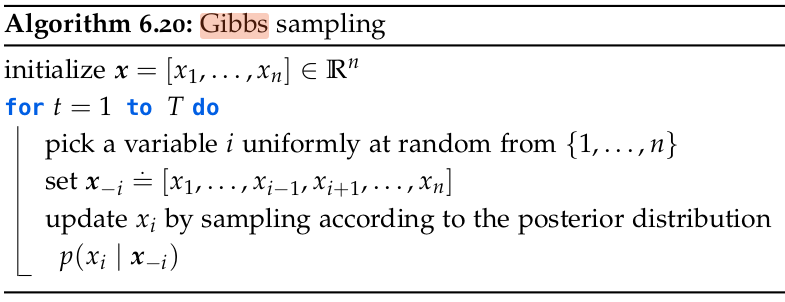
\includegraphics[width=0.98\linewidth]{images/Gibbs_Sampling.png} 
The stationary distribution of the simulated Markov chain is $p(\vx)$.
A \textbf{Gibbs distribution} is a continuous distribution $p$ whose PDF is of the form $p(\vx) = \frac{1}{Z} \exp(- f(\vx))$. $f$ is also called an \textbf{energy function}.
When the energy function $f$ is convex, its Gibbs distribution is called \textbf{log-concave distribution}. Can write: $\alpha(\vxp \mid \vx) = \min \braces*{1, \frac{r(\vx \mid \vxp)}{r(\vxp \mid \vx)} \exp(f(\vx) - f(\vxp))}$. \\
For $p(\vx) \propto \exp(-f(\vx))$: $\S{p(\vx)} = f(\vx) + \log Z$
\begin{framed}
    \textbf{Langevin Dynamics}: $r(\vxp \mid \vx) = \N[\vxp]{\vx - \eta_t \grad f(\vx)}{2 \eta_t \mI}$.
\textbf{MALA (Metropolis Adjusted Langevin Algorithm)}: Use Langevin dynamics with accept-reject step, mixing time polynomial in \(d\).
\textbf{SGLD (Stochastic Gradient Langevin Dynamics)}: Use Langevin dynamics, but always accept, and use stochastic gradients.
\end{framed}

\section{Bayesian Deep Learning}
\begin{framed}
    A deep \textbf{neural network} is a function: $\vf(\vx; \vtheta) \defeq \vvarphi(\mW_L \vvarphi(\mW_{L-1} ( \cdots \vvarphi(\mW_1 \vx))))$, where $\vtheta \defeq [\mW_1, \dots, \mW_L]$ is a vector of \textbf{weights}, and $\varphi : \R \to \R$ is a component-wise nonlinear \textbf{activation function}:\\
    $\mathrm{Tanh}(z) \defeq \frac{\exp(z) - \exp(-z)}{\exp(z) + \exp(-z)}$ \\
    $\mathrm{ReLU}(z) \defeq \max \{z, 0\} \in [0, \infty)$.
\end{framed}
\textbf{Softmax}: $\sigma_i(\vf) \defeq \frac{\exp(f_i)}{\sum_{j=1}^c \exp(f_j)}$ (classification)
\begin{framed}
    \textbf{Bayesian neural networks}: Gaussian prior on weights $\vtheta \sim \N{\vzero}{\sigmap^2 \mI}$, and Gaussian likelihood: \\
    $y \mid \vx, \vtheta \sim \N{f(\vx; \vtheta)}{\sigman^2}$. MAP estimate:\\
    $\vthetahat_\MAP = \argmin_\vtheta \frac{1}{2 \sigmap^2} \norm{\vtheta}_2^2 + \frac{1}{2 \sigman^2} \sum_{i=1}^n (y_i - f(\vx_i; \vtheta))^2$. Update rule: $\vtheta \gets \vtheta(1 - \frac{\eta_t}{\sigmap^2}) + \eta_t \sum_{i=1}^n \grad \log p(y_i \mid \vx_i, \vtheta)$
\end{framed}
\textbf{Heteroscedastic Noise}: Use a neural network with 2 outputs $f_1, f_2$, and define: $y \mid \vx, \vtheta \sim \N{\mu(\vx; \vtheta)}{\sigma^2(\vx; \vtheta)}$ where $\mu(\vx; \vtheta) \defeq f_1(\vx; \vtheta)$ and $\sigma^2(\vx; \vtheta) \defeq \exp(f_2(\vx; \vtheta))$.
$\log p(y_i \mid \vx_i, \vtheta) = \const - \frac{1}{2} \brackets*{\log \sigma^2(\vx_i; \vtheta) + \frac{(y_i - \mu(\vx_i; \vtheta))^2}{\sigma^2(\vx_i; \vtheta)}}$.
Approximate predictive distribution by sampling from the variational posterior $p(\ys \mid \vxs, \vx_{1:n}, \vy_{1:n}) \approx \E[\theta \sim q_\vlambda]{p(\ys \mid \vxs, \vtheta)}\approx \frac{1}{m} \sum_{i=1}^m p(\ys \mid \vxs, \vtheta^{(i)})$.

\section{Active Learning}
\begin{framed}
    \textbf{Conditional Entropy}: $\H{\rX \mid \rY} \defeq \E[\vy \sim p(\vy)]{\H{\rX \mid \rY = \vy}} \\= \E[(\vx, \vy) \sim p(\vx, \vy)]{- \log p(\vx \mid \vy)}$ \\
    \textbf{Joint entropy}: $\H{\rX, \rY} \defeq \E[(\vx, \vy) \sim p(\vx, \vy)]{- \log p(\vx, \vy)}$ 
    \vspace{1mm}
\end{framed}
\begin{framed}
    \textbf{Properties}: $\H{\rX, \rY} = \H{\rY} + \H{\rX \mid \rY} = \H{\rX} + \H{\rY \mid \rX}$ \\
    $\H{\rX \mid \rY} = \H{\rY \mid \rX} + \H{\rX} - \H{\rY}$ (Bayes Rule) \\
    $\H{\rX \mid \rY} \leq \H{\rX}$ (Information never hurts)
\end{framed}
\begin{framed}
    \textbf{Mutual Information}: $\I{\rX}{\rY} \defeq \H{\rX} + \H{\rY} - \H{\rX, \rY}$. Symmetric, $\leq$ 0. equal when X/Y independant.
\end{framed}
Have: $\I{\rX}{\rY} = \E[\vy \sim p]{\KL{p(\vx \mid \vy)}{p(\vx)}}$. \\
\textbf{Conditional mutual information}: $\I{\rX}{\rY}[\rZ] = \H{\rX \mid \rZ} - \H{\rX \mid \rY, \rZ}$. \\
$I(X; Y \mid Z) = I(X; Y, Z) - I(X; Z), \\ \quad I(X; Y; Z) = I(X; Y) - I(X; Y \mid Z)$ ($Y$ & $Z$ shared info on $X$). Symmetric; Positive $\rightarrow$ redundancy of $Y$ and $Z$ on $X$, Negative $\rightarrow$ synergy of $Y$ and $Z$ on $X$ (together $\gt$ their sums).

Given a (discrete) function $F : \pset{\spX} \to \R$, the \textbf{marginal gain} of $\vx \in \spX$ given $\sA \subseteq \spX$ is defined as $\Delta_F(\vx \mid \sA) \defeq F(\sA \cup \{\vx\}) - F(\sA)$. The function is called \textbf{submodular} iff for any $\vx \in \spX$ and any $\sA \subseteq \sB \subseteq \spX$ it satisfies $F(\sA \cup \{\vx\}) - F(\sA) \geq F(\sB \cup \{\vx\}) - F(\sB)$, it is called \textbf{monotone} it satisfies $F(\sA) \leq F(\sB)$. \\
\begin{framed}
    \textbf{Maximization objective}: monotone submodular function: \\ $I(\sS) \defeq \I{\vf_\sS}{\vy_\sS} = \H{\vf_\sS} - \H{\vf_\sS \mid \vy_\sS}$.
\end{framed}
\textbf{Greedy}: Pick the locations $\vx_1$ through $\vx_n$ individually by greedily finding the location with the maximal mutual information, this provides a $(1 - \nicefrac{1}{e})$-approximation of the optimum. Maximizing a subset's info gain otherwise is NP-hard.\\
\textbf{Uncertainty sampling}: Have already picked $\sS_t = \{\vx_1, \dots, \vx_t\}$; Solve the following: $\vx_{t+1} \defeq \argmax_{\vx \in \spX} \Delta_I(\vx \mid \sS_t) = \argmax_{\vx \in \spX} \Ism{f_\vx}{y_{\vx} \mid \vy_{\sS_t}}=\argmax_{\vx\in \spX}{\sigma_t^2(x)} $. Does not work with heteroscedastic noise, use \(\argmax_{\vx\in \spX} \frac{\sigma_t^2(x)}{\sigma_n^2(x)} \): large aleatoric uncertainty may dominate the epistemic uncertainty. In classification corresponds to selecting the label that maximizes the entropy of the predicted label: $\vx_{t+1} \defeq \argmax_{\vx \in \spX} \H{y_{\vx} \mid \vx_{1:t}, y_{1:t}}$. \\
\begin{framed}
    \textbf{Bayesian active learning by disagreement (BALD)}: This identifies those points $\vx$ where the models \emph{disagree} about the label $y_{\vx}$ (that is, each model is ``confident'' but the models predict different labels): $\vx_{t+1} \defeq \argmax_{\vx \in \spX} \I{\vtheta}{y_{\vx} \mid \vx_{1:t}, y_{1:t}} = \argmax_{\vx \in \spX} \H{y_{\vx} \mid \vx_{1:t}, y_{1:t}} - \E*[\vtheta \mid \vx_{1:t}, y_{1:t}]{\H{y_{\vx} \mid \vtheta}}$ 
\end{framed}

\section{Bayesian Optimization}
\begin{framed}
    The \textbf{Regret} for a time horizon $T$ associated with choices $\{\vx_t\}_{t=1}^T$ is defined as: $R_T \defeq \sum_{t=1}^T {\max_\vx \opt{f}(\vx) - \opt{f}(\vx_t)}$.
\end{framed}
Goal: sublinear regret: $\lim_{T\to\infty} \frac{R_T}{T} = 0$.
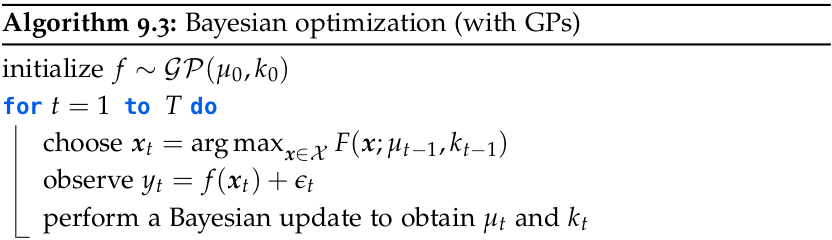
\includegraphics[width=0.98\linewidth,trim={0 0 3cm 0}]{images/Bayesian_Optimization.png}
Use \textbf{acquisition function} to greedily pick the next point to sample based on the current model. \\
\textbf{Upper confidence bound}: $\vx_{t+1} \defeq \argmax_{\vx \in \spX} \mu_{t}(\vx) + \beta_{t+1} \sigma_{t}(\vx)$, where $\sigma_t(\vx) \defeq \sqrt{k_t(\vx, \vx)}$. If $\beta_t = 0$ then UCB is purely exploitative; if $\beta_t \to \infty$, UCB recovers uncertainty sampling.
\begin{framed}
    Choosing $\beta_t$ appropriately we get: $R_T = \BigO{\sqrt{T \gamma_T}}$, where $\gamma_T \defeq \max_{\substack{\sS \subseteq \spX \\ \card{\sS} = T}} \I{\vf_\sS}{\vy_\sS} = \max_{\substack{\sS \subseteq \spX \\ |\sS| = T}} \frac{1}{2} \log\det{\mI + \sigman^{-2} \mK_{\sS\sS}}$, is the maximum information gain after $T$ rounds.
\end{framed}
\begin{framed}
    \textbf{Information gain of some kernels}:
    Linear: $\gamma_T = \BigO{d \log T}$ \\
    Gaussian: $\gamma_T = \BigO{(\log T)^{d+1}}$ \\
    Matérn $\nu > \frac{1}{2}$: $\gamma_T = \BigO{T^{\frac{d}{2\nu + d}} (\log T)^{\frac{2\nu}{2\nu + d}}}$
\end{framed}
\textbf{Thompson Sampling}: At time $t+1$, we sample a function $\Tilde{f}_{t+1} \sim p(\cdot \mid \vx_{1:t}, y_{1:t})$ from our posterior distribution.
Then, we simply maximize $\Tilde{f}_{t+1}$, $\vx_{t+1} \defeq \argmax_{\vx \in \spX} \Tilde{f}_{t+1}(\vx)$.

\section{Markov Decision Processes}
\begin{framed}
    A \textbf{(finite) Markov decision process} is specified by a (finite) set of \textbf{states} $\sX \defeq \{1, \dots, n\}$; a (finite) set of \textbf{actions} $\sA \defeq \{1, \dots, m\}$; \textbf{transition probabilities} ${p(x' \mid x, a) \defeq \Pr{X_{t+1} = x' \mid X_t = x, A_t = a}}$; a \textbf{reward function} $r : X \times A \to \R$ which maps the current state $x$ and an action $a$ to some \textbf{reward}.
\end{framed}
$r$ induces a sequence of rewards: $R_t \defeq r(X_t, A_t)$.
\begin{framed}
    A \textbf{policy} is a function that maps each state $x \in \sX$ to a probability distribution over the actions. That is, for any $t > 0$: $\pi(a \mid x) \defeq \Pr{A_t = a \mid X_t = x}$.
\end{framed}
A policy induces a MC $(X_t^\pi)_{t\in\Nat_0}$: $p^\pi(x' \mid x) \defeq \Pr{X_{t+1}^\pi = x' \mid X_t^\pi = x} = \sum_{a \in \sA} \pi(a \mid x) p(x' \mid x, a)$.\\
The \textbf{discounted payoff} from time $t$ is: $G_t \defeq \sum_{m=0}^\infty \gamma^m R_{t+m}$, for $\gamma \in [0, 1)$, the \textbf{discount factor}.
\begin{framed}
    The \textbf{state value function}: $\E[\pi]{\cdot} \defeq \E[(X_t^\pi)_{t\in\Nat_0}]{\cdot}$ measures the average discounted payoff from time $t$ starting from state $x \in \sX$.
\end{framed}
\begin{framed}
    The \textbf{state-action value function (Q-function)}: $\q[\pi]{x}{a}[t] \defeq \E[\pi]{G_t \mid X_t = x, A_t = a} = r(x, a) + \gamma \sum_{x' \in \sX} p(x' \mid x, a) \cdot \v[\pi]{x'}[t+1]$ measures the average discounted payoff from time $t$ starting from state $x \in \sX$ and with playing action $a \in \sA$.
\end{framed}
\begin{framed}
    \textbf{Bellman Expectation Equation}: $\v[\pi]{x} = r(x, \pi(x)) + \gamma \E[x' \mid x, \pi(x)]{\v[\pi]{x'}}$, if stochastic policy: $\v[\pi]{x} = \E[a \sim \pi(x)]{\q[\pi]{x}{a}}$. Also get: $\q[\pi]{x}{a} = r(x, a) + \gamma \E*[x' \mid x, a]{\E[a' \sim \pi(x')]{\q[\pi]{x'}{a'}}}$. For deterministic: $\v[\pi]{x} = \q[\pi]{x}{\pi(x)}$.
\end{framed}
Can be used to find $\fnv[\pi]$ given policy $\pi$, by solving linear system of equations in cubic time in the size of the state space. Can also be solved using fixed point iteration: $\mB^\pi \vv \defeq \vr^\pi + \gamma \mP^\pi \vv$.
\begin{framed}
    A \textbf{greedy policy} w.r.t. to a state-action value function $\fnq$ is $pi_{\fnq}(x) \defeq \argmax_{a \in \sA} \q{x}{a}$; a \textbf{greedy policy} w.r.t. a state value function $\fnv$ is: $\pi_{\fnv}(x) \defeq \argmax_{a \in \sA} r(x, a) + \gamma \sum_{x' \in \sX} p(x' \mid x, a) \cdot \v{x'}$.
\end{framed}
\begin{framed}
    \textbf{Bellman's Theorem}: A policy $\pis$ is optimal iff it is greedy with respect to its own value function. In other words, $\pis$ is optimal iff $\pis(x)$ is a distribution over the set $\argmax_{a \in \sA} \q*{x}{a}$.
\end{framed}
If or every state there is a unique action that maximizes the state-action value function, the policy $\pis$ is deterministic and unique, $\pis(x) = \argmax_{a \in \sA} \q*{x}{a}$.
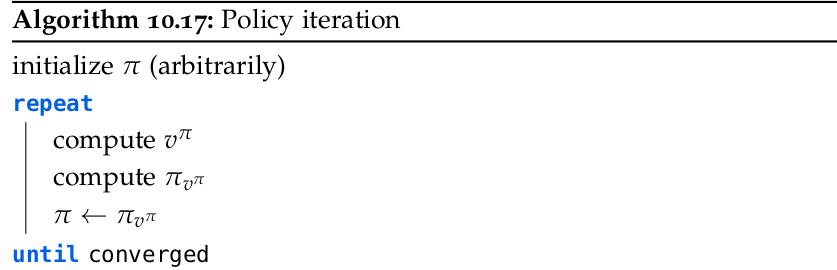
\includegraphics[width=\linewidth, trim={0 0 3cm 0}]{images/Policy_Iteration.png}
For finite Markov decision processes, policy iteration converges to an optimal policy.
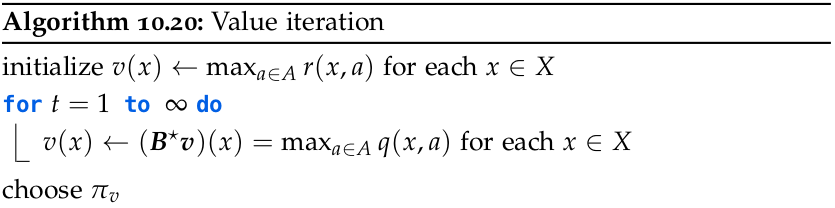
\includegraphics[width=\linewidth, trim={0 0 3cm 0}]{images/Value_Iteration.png}
Value iteration converges to an optimal policy, as $\fnv[\star]$ and $\fnq[\star]$ are a fixed-points of the Bellman update $\mBs$.
\begin{framed}
    A \textbf{Partially observable Markov decision process (POMDP)} is a Markov process, with a set of supplementary \textbf{observations} $\sY$, and \textbf{observation probabilities} $o(y \mid x) \defeq \Pr{Y_t = y \mid X_t = x}$.
\end{framed}
POMDP are hard to solve in general, but can be reduced to MDP with an enlarged state space. We consider MDP whose state are \textbf{beliefs}: $b_t(x) \defeq \Pr{X_t = x \mid y_{1:t}, a_{1:t-1}}$. Keeping track of how beliefs change over time is \textbf{Bayesian filtering}: Given a prior belief $b_t$, an action taken $a_t$, and a new observation $y_{t+1}$, the belief state can be updated as: $b_{t+1}(x) = \Pr{X_{t+1} = x \mid y_{1:t+1}, a_{1:t}} = \frac{1}{Z} o(y_{t+1} \mid x) \sum_{x' \in \sX} p(x \mid x', a_t) b_t(x')$, where $Z \defeq \sum_{x \in \sX} o(y_{t+1} \mid x) \sum_{x' \in \sX} p(x \mid x', a_t) b_t(x')$.
The sequence of belief-states defines the sequence of random variables $(B_t)_{t\in\Nat_0}$:$ B_t \defeq X_t \mid y_{1:t}, a_{1:t-1}$, where the (state-)space of all beliefs is the (infinite) space of all probability distributions over $\sX$: $\spB \defeq \Delta^{\sX} \defeq \braces*{\vb \in \R^{\card{\sX}} : \vb \geq \vzero, \textstyle\sum_{i=1}^{\card{\sX}} \vb(i) = 1}$.
\begin{framed}
    Given a POMDP, the corresponding \textbf{Belief-state Markov decision process} is a Markov decision process specified by the \textbf{belief space} $\spB \defeq \Delta^{\sX}$ depending on the \textbf{hidden states} $\sX$; the set of \textbf{actions} $\sA$; \textbf{transition probabilities} $\tau(b' \mid b, a) \defeq \Pr{B_{t+1} = b' \mid B_t = b, A_t = a}$; and \textbf{rewards} $\rho(b, a) \defeq \E[x \sim b]{r(x, a)} = \sum_{x \in \sX} b(x) r(x, a)$.
\end{framed}
Have: $\tau(b_{t+1} \mid b_t, a_t) = \Pr{b_{t+1} \mid b_t, a_t} = \sum_{y_{t+1} \in \sY} \Pr{b_{t+1} \mid b_t, a_t, y_{t+1}} \Pr{y_{t+1} \mid b_t, a_t}$. We also set: $\Pr{b_{t+1} \mid b_t, a_t, y_{t+1}} = 1$ iff $b_{t+1}$ matches the belief update given $b_t, a_t$, and $y_{t+1}$, and 0 else. Finally the likelihood is: $\Pr{y_{t+1} \mid b_t, a_t} = \E[x \sim b_t]{\E[x' \mid x, a_t]{\Pr{y_{t+1} \mid X_{t+1} = x'}}} = \sum_{x \in \sX} b_t(x) \sum_{x' \in \sX} p(x' \mid x, a_t) \cdot o(y_{t+1} \mid x')$.
\section{Tabular Reinforcement Learning}

A trajectory $\tau$ is a sequence: $\tau \defeq (\tau_0, \tau_1, \tau_2, \dots)$, with $\tau_i \defeq (x_i, a_i, r_i, x_{i+1})$.
Agent can choose any policy $\rightarrow$ \textbf{on-policy} method. \\
No choice of policy $\rightarrow$ \textbf{off-policy} method. \\
\textbf{Model-based} $\rightarrow$ Learn the underlying MDP \\
\textbf{Model-free} $\rightarrow$ Learn value function directly.
All model-based methods are off-policy.
\begin{framed}
    \textbf{RM conditions}: $\alpha_t \geq 0$, $\sum_{t=0}^{\infty}{\alpha_t} = \infty$, $\sum_{t=0}^{\infty}{\alpha_t^2} < \infty$.
\end{framed}
\begin{framed}
    \textbf{Monte Carlo Control}
    Estimate underlying MDP using Monte carlo estimation:
    ${\hat{p}(x' \mid x, a) = \frac{N(x' \mid x, a)}{N(a \mid x)}}$ and \\ ${\hat{r}(x, a) = \frac{1}{N(a \mid x)} \sum_{t = 0, x_t = x,a_t = a}^\infty r_t}$
\end{framed}
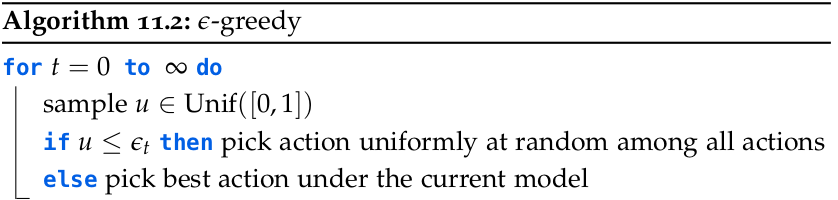
\includegraphics[width=0.95\linewidth,trim={0 0 3cm 0}]{images/epsilon_greedy.png}
\(\varepsilon\)-greedy converges to the optimal policy if the RM conditions are satisfied for \(\varepsilon_t\) and all state-action pairs are visited infinitely often.
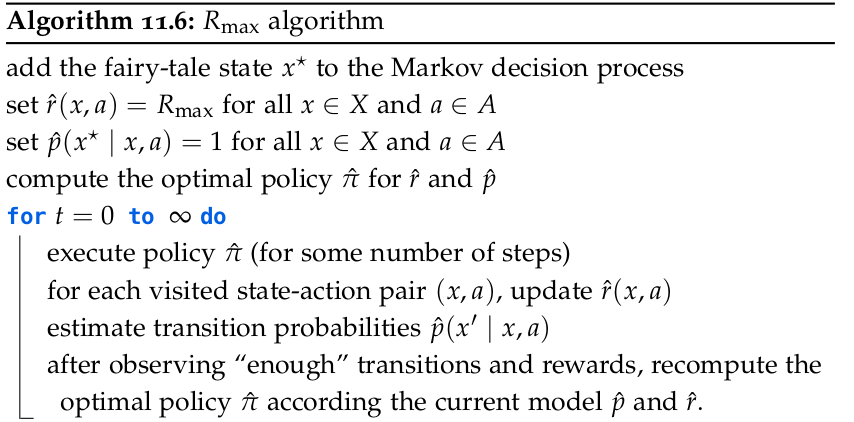
\includegraphics[width=0.95\linewidth, trim={0 0 3cm 0}]{images/R_max.png}
With probability at least $1-\delta$, $R_\mathrm{max}$ reaches an $\epsilon$-optimal policy in a number of steps that is polynomial in $\card{\sX}$, $\card{\sA}$, $T$, $\nicefrac{1}{\epsilon}$, $\nicefrac{1}{\delta}$, and $R_\mathrm{max}$.
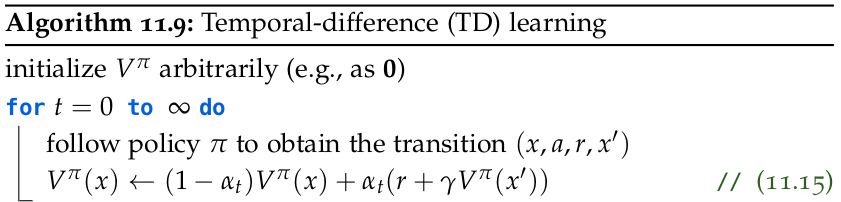
\includegraphics[width=0.95\linewidth,trim={0 0 4cm 0}]{images/TD_learning.png}
This is an on-policy method.
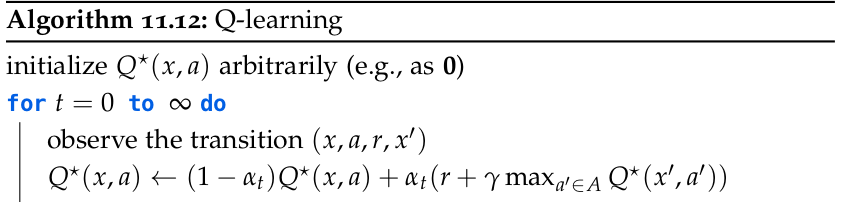
\includegraphics[width=0.95\linewidth, trim={0 0 3cm 0}]{images/Q_learning.png}
This is an off-policy method.
Optimistic: init $Q(x,a) = \frac{R_{\max}}{1-\gamma}$ for all $(x,a)$ pairs.
The update rule can also be expressed as: $\Q*{x}{a} \gets \Q*{x}{a} + \alpha_t\parentheses*{r + \gamma \max_{a' \in \sA} \Q*{x'}{a'} - \Q*{x}{a}}$.
Both converge if $\alpha_t$ satisfy RM conditions and every state-action pair is visited infinitely often.
RM: \(\alpha_t > 0, \sum_{t=1}^\infty \alpha_t = \infty, \sum_{t=1}^\infty \alpha_t^2 < \infty\). (Step sizes diminish but not too quickly.)

%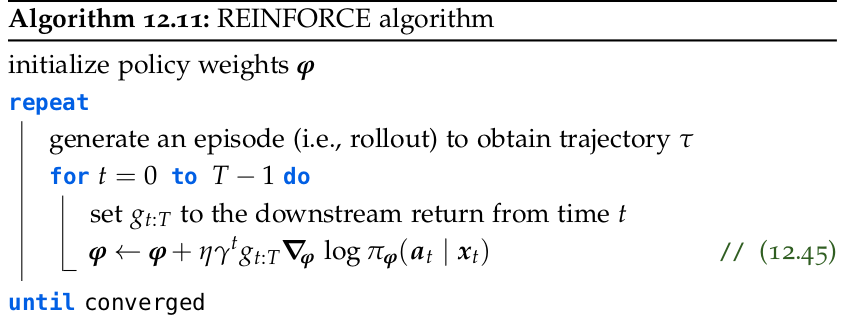
\includegraphics[width=\linewidth]{images/REINFORCE.png}

\section{Model-free Reinforcement Learning}
Can view TD-learning as SGD on the squared loss $\ell(\vtheta; x, r, x') \defeq \frac{1}{2}\parentheses*{r + \gamma \old{\vtheta}(x') - \vtheta(x)}^2$. 
The gradient of this loss is called TD error, \(\delta_{\mathrm{TD}}=\grad_{\vtheta(x)}\ell(\vtheta; x, r, x')=\vtheta(x)-(r+\gamma\theta^{\mathrm{old}}(x'))\) \\
\textbf{Parametric value function approximation}: To scale to large state spaces, learn approximation
of (action) value function $\V{\vx; \vtheta}$ or $\Q{\vx}{\va; \vtheta}$. For e.g. the parameters $\vtheta$ of a neural network.
\begin{framed}
    \textbf{Q-learning with function approximation}: In state $\vx$, pick action $a$; Observe $\vx'$, reward $r$. Update $\vtheta \gets \vtheta + \alpha_t \delta_\mathrm{B} \grad_\vtheta Q^*(\vx, \va; \vtheta)$, where $\delta_\mathrm{B} \defeq r + \gamma \max_{\vap \in \spA} \Q*{\vxp}{\vap; \old{\vtheta}} - \Q*{\vx}{\va; \vtheta}$.
\end{framed}
\begin{framed}
    \textbf{Deep Q Networks}
    Use replay buffer of size \(|\mathcal{D}|\): \(\ell_{\mathrm{DQN}}(\vtheta; \mathcal{D})=\frac{1}{2}\sum_{(\vx, \va, r, \vx')\in \mathcal{D}}{(r+\gamma \max_{\va'\in \mathcal{A}}Q^*(\vx',\va'; \vtheta^{\mathrm{old}})}-Q^*(\vx,\va;\vtheta))^2\)
\end{framed}
\begin{framed}
    \textbf{Double Deep Q Networks}
    Loss function of DQN uses noisy estimate of \(q^*\), leading to a biased estimate of  \(\max\ q^*\).
    Instead of picking the optimal action with respect to the old network, pick the optimal action with respect to the new network, \(\va^*(\vx';\vtheta)=\argmax_{\va'\in \mathcal{A}} Q^*(\vx',\va';\vtheta), \ell_{\mathrm{DDQN}}(\vtheta; \mathcal{D})=\frac{1}{2}\sum_{(\vx, \va, r, \vx')\in \mathcal{D}}{(r+\gamma Q^*(\vx',a^*(\vx';\vtheta); \vtheta^{\mathrm{old}})}-Q^*(\vx,\va;\vtheta))^2\)
\end{framed}
\begin{framed}
    The \textbf{policy value function} measures the discounted payoff of policy $\pi$: $\j{\pi} \defeq \E[\pi]{G_0} = \E[\pi]{\sum_{t=0}^\infty \gamma^t R_t}$, and the bounded variant: $\j{\pi}[T] \defeq \E[\pi]{G_{0:T}} = \E[\pi]{\sum_{t=0}^{T-1} \gamma^t R_t}$. Abbreviate $\j{\vvarphi} \defeq \j{\pi_\vvarphi}$
\end{framed}
\begin{framed}
    \textbf{Score Gradient Estimator} \\
    \(\grad_{\varphi}\mathbb{E}_{\tau\sim\Pi_{\varphi}}[G_0]=\mathbb{E}_{\tau\sim\Pi_{\varphi}}[G_0 \grad_{\varphi} \log \Pi_{\varphi}(\tau)]\)\\
    We have \(\grad_{\varphi} \log \Pi_{\varphi}(\tau)=\sum_{t=0}^{T-1}{\grad_{\varphi}\pi_{\varphi}(\va_t\mid \vx_t)}\)

\end{framed}
\begin{framed}
    \textbf{Baselines}\\ For \(b\in \mathbb{R}\), $\mathbb{E}_{\tau\sim\Pi_{\varphi}}[G_0 \grad_{\varphi} \log \Pi_{\varphi}(\tau))=\mathbb{E}_{\tau\sim\Pi_{\varphi}}[(G_0-b) \grad_{\varphi} \log \Pi_{\varphi}(\tau))$.
    This holds true, even for baselines depending on \textit{previous} states.
\end{framed}
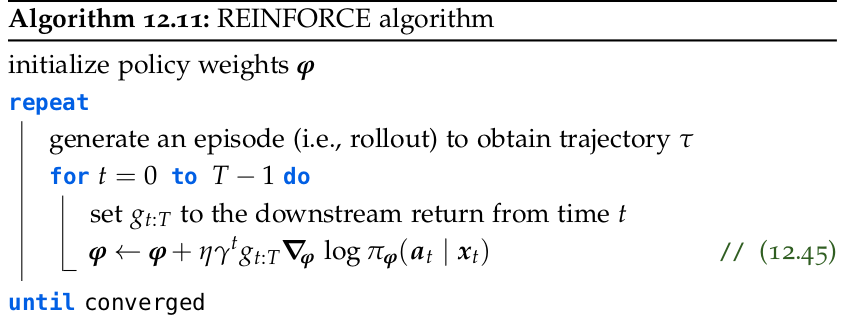
\includegraphics[width=\linewidth]{images/REINFORCE.png}
\begin{framed}
    Given a policy $\pi$, the \textbf{advantage function} is $\a[\pi]{\vx}{\va} \defeq \q[\pi]{\vx}{\va} - \v[\pi]{\vx} = \q[\pi]{\vx}{\va} - \E[\vap \sim \pi(\vx)]{\q[\pi]{\vx}{\vap}}$
\end{framed}
$\text{$\pi$ is optimal} \iff \forall \vx \in \spX, \va \in \spA : \a[\pi]{\vx}{\va} \leq 0$
\begin{framed}
    \textbf{Policy Gradient Theorem}\\
    The policy gradient can be represented in terms of the Q-function: \(\grad_{\varphi}{j(\varphi)}=\sum_{t=0}^{\infty}{\mathbb{E}_{\vx_t,\va_t}[\gamma^t q^{\pi_\varphi}(\vx_t,\va_t)\grad_\varphi \log \pi_{\varphi}(\va_t\mid \vx_t)]}\).

    
\end{framed}
\begin{framed}
  \textbf{Actor-Critic methods} consist of two components: a parameterized policy, $\pi(\va \mid \vx; \vvarphi) \eqdef \pi_\vvarphi$, which is called \textbf{actor}; and a value function approximation, $\q[\pi_\vvarphi]{\vx}{\va} \approx \Q[\pi_\vvarphi]{\vx}{\va; \vtheta}$, which is called \textbf{critic}.
\end{framed}
%Use gradient approximation: 
%\tiny{$\grad_\vvarphi \J{\vvarphi} \approx \sum_{t=0}^\infty\E[(\vx_t,\va_t) \sim \pi_\vvarphi]{\gamma^t \Q{\vx_t}{\va_t; \vtheta} \grad_\vvarphi \log \pi_\vvarphi(\va_t \mid \vx_t)}$}
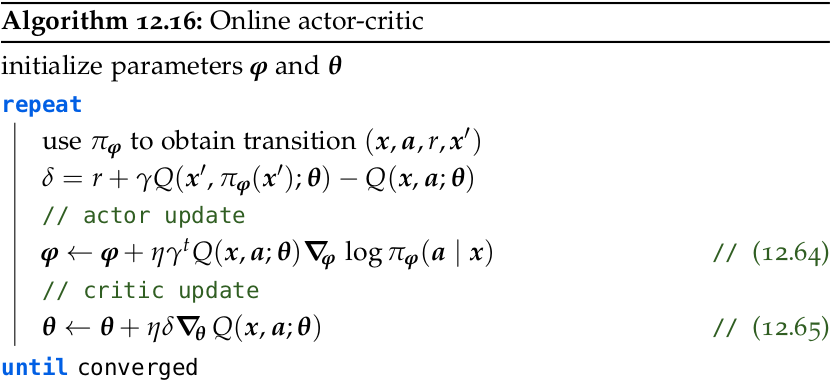
\includegraphics[width=0.95\linewidth, trim={0 0 4cm 0}, height=2.5cm]{images/Online_actor_critic.png}
\begin{framed}
    \textbf{Maximum Entropy Reinforcement Learning}
    Encourage exploration by regularizing policies towards uncertainty: \(j_{\lambda}(\varphi)=j(\varphi)+\lambda \H{\Pi_{\varphi}}\).
\end{framed}

\section{Model-based Reinforcement Learning}

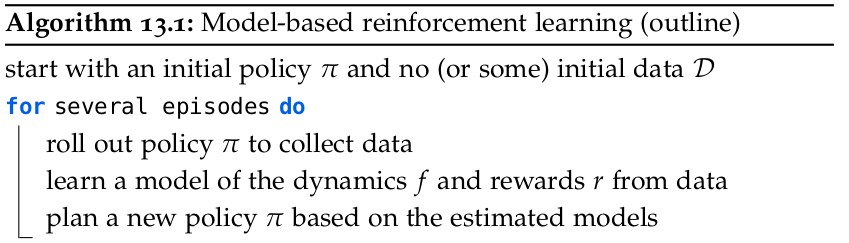
\includegraphics[width=0.95\linewidth, ,trim={0 0 3cm 0}]{images/Model_based_reinforcement_learning.png}
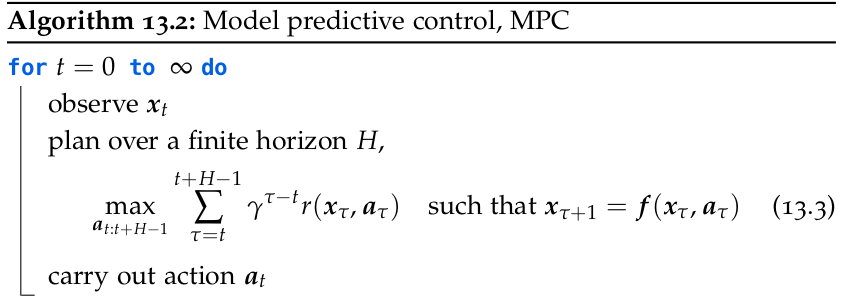
\includegraphics[width=0.95\linewidth,trim={0 0 3cm 0}]{images/MPC.png}
By Nils Jensen --- nils.jensen@inf.ethz.ch --- HS2023
\end{multicols*}
\end{document}
